\chapter{Исследование методов и средств  формирования CAPAs на основе изменений репозитория кода} \label{ch1}

\section{Современные подходы к формированию CAPA на основе анализа репозиториев кода} \label{ch1:sec1}

Корректирующие и предупреждающие действия CAPA представляют собой ключевой элемент систем управления качеством, направленных на выявление и устранение дефектов, а также предупреждение их повторного возникновения [\ref{FDA}]. Изначально применяемые в регулируемых отраслях (медицина, фармацевтика и т.д.), концепции CAPA становятся актуальными и для разработки программного обеспечения, где цель сводится к автоматизации обнаружения проблем в коде и предложению мер по их исправлению или предотвращению. В контексте анализа изменений в репозиториях кода задача формирования CAPA сводится к систематическому анализу истории коммитов, метрик и паттернов изменений с целью выявления аномалий и генерации рекомендаций для разработчиков.

Существует несколько направлений и инструментов, применимых к этой задаче. Одни ориентированы на управление качеством как таковым (системы QMS и CAPA-менеджмента), другие – на технический анализ исходного кода и истории версий (статический анализ, JIT-предсказание дефектов, классификация коммитов). Современные подходы активно используют методы машинного обучения и искусственного интеллекта для выявления закономерностей в репозиториях и автоматической генерации CAPA [\ref{Bugayenko2022}][\ref{Commit-classification}]. В этой главе рассматриваются существующие модели и инструменты, а также их сравнение по критериям автоматизации, интеграции в CI/CD, применимости к истории коммитов и интерпретируемости результатов.

\section{Системы управления CAPA и интеграция в процессы разработки} \label{ch1:sec2}

В классических системах контроля качества (например, ISO 9001, FDA 21 CFR Part 820) CAPA оформляются документально и отслеживаются средствами QMS. Такие системы (Quality Management Systems) обеспечивают формализацию процесса: сбор инцидентов, расследование причин, планирование и выполнение действий, верификацию эффективности. Большинство коммерческих решений по CAPA (Qualityze, MasterControl, SimplerQMS и т.д.) предлагают удобные интерфейсы для заполнения карточек CAPA и управления ими, но они не заточены под анализ кода или репозиториев. Автоматизация в этих системах ограничена триггерами (например, создание CAPA на основе записи о сбое теста или жалобы), и интеграция с процессами CI/CD чаще всего осуществляется через ручные интерфейсы или API. Подходы такого рода обеспечивают качественный учет проблем и статус выполнения мер, однако они не анализируют непосредственно изменения в коде и не извлекают CAPA автоматически на основе метрик репозитория [\ref{FDA}].

Напротив, современные инструментальные решения в области разработки ПО стремятся к раннему обнаружению проблем в процессе написания кода. Сюда относятся системы статического анализа кода (SonarQube, CodeQL, Coverity), инструменты анализа сборок и покрытий (Codecov), а также инструменты анализа истории версий и производительности (Pluralsight Flow, CodeScene и др.). Такие инструменты обычно легко интегрируются в конвейер CI/CD (GitLab CI, Jenkins, GitHub Actions и др.), автоматизированно собирают метрики кода и могут генерировать отчеты с найденными дефектами или подозрениями. Например, SonarQube при подключении к Git-серверу автоматически анализирует каждый коммит или пулл-реквест на наличие проблем (code smells, багов, уязвимостей) и может предлагать меры по их устранению. Выходные данные статических анализаторов часто имеют стандартизированный формат (например, SARIF – Static Analysis Results Interchange Format), что облегчает интеграцию и агрегирование результатов [\ref{FDA}]. Недостатком здесь является то, что такие инструменты обычно фокусируются на анализе текущего состояния кода, но не делают выводов о процессе разработки в целом или о трендах аномалий в истории коммитов. Тем не менее, их отчеты служат основой для корректирующих действий (исправление найденных дефектов) и косвенно могут стимулировать превентивные меры по устранению проблем.

\section{Методы анализа коммитов и обучение на данных репозиториев} \label{ch1:sec3}
\subsection{Предсказание дефектных коммитов}
Одним из популярных подходов в анализе изменений является Just-In-Time Software Defect Prediction (JIT-SDP), направленный на обнаружение потенциально «багогенерирующих» коммитов до интеграции изменений. Модели JIT-SDP строятся на исторических данных о прошлых коммитах (метриках изменений, метаданных, сообщениях к коммитам) и обучаются классифицировать новые коммиты как безопасные или потенциально дефектные. Например используя метод одно-классовой классификации для идентификации аномалий среди коммитов [\ref{One-Class}]. Для её реализации модель обучается на «нормальных» (не дефектных) коммитах и затем помечает отклонения как подозрительные. Эксперименты показали, что при высоком дисбалансе классов (мало баговых коммитов относительно нормальных) одно-классовые алгоритмы (One-Class SVM, Isolation Forest и т.д.) превосходят традиционные классификаторы по точности обнаружения дефектных изменений [\ref{One-Class}]. JIT-SDP можно встроить непосредственно в систему контроля версий: модель принимает данные о новом коммите при попытке его зафиксировать и возвращает прогноз (например, в виде уведомления разработчику), что позволяет принять коррективные действия (дополнительная проверка, тестирование) до слияния. Такие подходы полностью автоматизированы (после первоначального обучения) и могут работать в CI/CD без вмешательства человека. Однако они часто ограничены точностью модели и могут давать ложные срабатывания, поэтому вопрос интерпретируемости результатов здесь актуален: разработчикам важно понимать, какие особенности коммита вызвали подозрение. Для повышения интерпретируемости предлагаются методы объяснения предсказаний (например, SHAP/ LIME или специальные эксплейнеры для JIT-SDP), хотя это выходит за рамки базовых моделей [\ref{One-Class}]. 

\subsection{Классификация коммитов по типам работ (Commit Classification)}

Другой распространённый подход – классификация коммитов по видам технических действий (например, категориальное разделение на корректирующие, адаптивные, совершенствующие задачи). Этот метод чаще используется для анализа уже сделанных изменений с целью обзора тенденций и построения рекомендаций. В литературе выделяют три классических типа изменений: Corrective (исправление дефектов), Adaptive (обработка требований/увеличение функциональности) и Perfective (улучшение производительности/рефакторинг) [\ref{Commit-classification}]. Основные характеристики таких моделей: они используют признаковые описания коммитов (количество строк, слова из сообщений, данные о затронутых файлах) и типичные алгоритмы машинного обучения (Decision Tree, Random Forest, Naive Bayes, нейросети) [\ref{Commit-classification}]. Результаты таких классификаторов помогают в формировании превентивных мер: например, если обнаруживается, что большое число коммитов носит корректирующий характер из-за недостаточного тестового покрытия, система может рекомендовать усилить модульное тестирование. В последние годы к этой задаче привлекаются большие языковые модели. Например, GPT-3 может в режиме zero-/few-shot эффективно классифицировать сообщения коммитов по категориям технической поддержки []\ref{Commit-classification}]. В частности, достигается \verb|~75%| точности классификации  по трём категориям [\ref{Commit-classification}].
Это свидетельствует о высокой автоматизируемости такого подхода и возможности использования предобученных моделей, однако интерпретируемость итоговых меток, особенно при применении LLM остается проблемой.

Классификаторы коммитов в целом демонстрируют высокую применимость к истории репозиториев, поскольку анализируют каждое изменения во временной последовательности. Они хорошо интегрируются в CI/CD и инструменты мониторинга (через плагины GitHub/GitLab) – фактически после фиксации коммита производится моментальная классификация с логированием результата. Однако такие системы требуют обширных размеченных данных для обучения (или хорошо сформулированных правил) и могут не учесть все контексты проекта, что снижает их точность для разных проектов [\ref{Commit-classification}][\ref{Sazid}]. Тем не менее, при правильной настройке они позволяют формировать CAPA как в корректирующей, так и превентивной части: например, классифицируя «адаптивные» коммиты, можно обнаружить систематические изменения в требованиях и заранее планировать архитектурные доработки.

\section{Инструменты и системы автоматизации CAPA} \label{ch1:sec4}

На практике для генерации CAPA в области разработки ПО применяются комбинированные решения, объединяющие анализ кода и процесс управления. Некоторые примеры:

\begin{itemize}
	\item Встроенные боты и скрипты в репозиторий. 
	
	Примером является система TOM (Theoretically Objective Measurements), описанная Bugayenko  и соавторами [\ref{Bugayenko2022}]. Для её использования необходимо лишь добавить бота @0capa в репозиторий. Он автоматически собирает метрики по каждому коммиту и на их основе предлагает CAPA. Такой подход максимально автоматизирован и интегрируется через механизмы GitHub (было реализовано создание pull request с рекомендациями CAPA). Информация о том, какие действия требует каждый коммит, хранится вместе с кодом, что повышает прозрачность процесса. Хоть и система была описана, готового решения по @0capa нет в открытом доступе.
	
	\item Плагины и дополнения к системам CI/CD.
	
	Многие CI-системы (GitLab, Jenkins, GitHub Actions) поддерживают установку плагинов, выполняющих анализ коммитов или статический анализ. Например, SonarQube имеет плагин SonarScanner для GitLab CI, а GitHub Actions – для автоматического запуска анализа при каждом PR. Некоторые сервисы (например, bugasura.io) предлагают «AI-инспектора», который отслеживает журналы сборок и автоматически сигнализирует о паттернах отказов. Такие инструменты часто обеспечивают интеграцию в процесс разработки и могут генерировать тикеты или отчеты CAPA. Форматы вывода обычно совместимы со стандартными трекерами (JIRA, GitHub Issues), что облегчает стандартизацию.
	
	\item Инструменты анализа pull-реквестов и метаданных.
	
	Существуют системы, которые обучены классифицировать Pull Request как «корректирующий» или «не корректирующий» [\ref{Bugayenko2022}]. По результатам анализа PR или истории веток такие инструменты могут «присваивать» CAPA к прошедшим исправлениям и накапливать статистику.  Это позволяет накапливать базу знаний о типичных рекомендациях и соотносить их с шаблонами изменений. Однако подобные решения пока редко встречаются в свободном доступе и требуют развитой инфраструктуры данных. [\ref{Bugayenko2022}]
	\item Статические анализаторы с функцией CAPA. 
	
	 Ряд современных SAST-инструментов (Fortify, Checkmarx, SonarQube) начинают включать в отчеты «рекомендации» помимо указания на проблему. Например, при обнаружении уязвимости система может автоматически предложить типовую корректирующую меру (обновить библиотеку, изменить код), что можно рассматривать как CAPA в узком смысле. Хотя это скорее рекомендации на уровне кода, а не на уровне процесса разработки, их вывод можно экспортировать для дальнейшей автоматической обработки. Интеграция в CI/CD у подобных систем хорошо налажена, а результаты достаточно интерпретируемы (описаны правила, чек-листы).
\end{itemize}

Таким образом, современные инструменты сходятся на том, что интеграция в процессы CI/CD и автоматизация – ключевое требование. Боты и плагины обеспечивают автоматический сбор данных из репозиториев и формирование CAPA-рекомендаций без участия человека, хотя зачастую требуют первоначальной настройки моделей и правил. Статические анализаторы обеспечивают проверку качества кода по стандартным правилам, и их выходы можно использовать для инициирования CAPA в QMS (например, через настройку связей с Jira или другой системой учета).



\begin{table}[htbp]
	\centering
	\caption{Сравнение инструментов формирования CAPA}
	\label{tab:capa_tools}
	\resizebox{\textwidth}{!}{%
		\begin{tabular}{|p{3cm}|p{2.6cm}|p{3cm}|p{3cm}|p{3cm}|p{3.6cm}|p{2.6cm}|p{2.6cm}|}
			\hline
			\shortstack[l]{\textbf{Решение}\\\textbf{}} &
			\shortstack[l]{\textbf{Инструмент}\\\textbf{}} &
			\shortstack[l]{\textbf{Открытый}\\\textbf{исходный код}} &
			\shortstack[l]{\textbf{CI/CD}\\\textbf{интеграция}} &
			\shortstack[l]{\textbf{Анализ}\\\textbf{истории}\\\textbf{коммитов}} &
			\shortstack[l]{\textbf{Статический}\\\textbf{анализ кода}\\\textbf{}} &
			\shortstack[l]{\textbf{Автовыдача}\\\textbf{CAPA}} &
			\shortstack[l]{\textbf{Формат}\\\textbf{CAPA}} 
			\\
			\hline
			MasterControl CAPA &
			QMS платформа &
			Нет &
			Нет &
			Нет &
			Нет &
			Осуществля-
			ется вручную &
			Полный аудит \\
			\hline
			CommitGuru &
			JIT-Defect Prediction &
			Да &
			Нет &
			Да &
			Частично &
			Да &
			Только степень риска,
			вероятность дефекта
			\\
			\hline
			@0capa (TOM) &
			Бот-анализ репозитория &
			Частично &
			Да &
			Да &
			Линтеры &
			Автомати-
			ческая
			Pull-Request &
			Текстовые шаблонные советы\\
			\hline
			Bugasura.io &
			CI-logs AI-inspector &
			Нет &
			Да &
			Нет &
			ESLint &
			Автомати-
			ческая Issue &
			Текстовые рекомендации при сбоях\\
			\hline
			Разрабатывае-
			мое 
			решение &
			ML-анализ коммитов и статический анализ &
			Да &
			Да (интеграция через CI/CD пайплайны) &
			Да (анализ истории коммитов) &
			Да (Pylint, Checkstyle, ESLint и др.) &
			Автоматичес-
			кая генерация рекомендаций CAPA &
			Подробные рекомендации с приоритетами и причинами риска \\
			\hline
		\end{tabular}%
	}
\end{table}

Ниже — текстовое описание каждого из выбранных критериев сравнения инструментов формирования CAPA:


Подход. Определяет алгоритмическую или организационную основу, на которой построен инструмент. QMS-платформа (MasterControl CAPA) реализует классический жизненный цикл CAPA: сбор инцидента, расследование, план действий, проверка эффективности. JIT-Defect Prediction (CommitGuru) — модель, обученная на истории коммитов, предсказывает «риск» в момент фиксации изменений. Бот-анализ репозитория (@0capa/TOM) — GitHub-App, который на каждый пуш автоматически собирает метрики и создаёт PR с рекомендациями. CI-logs AI-inspector (Bugasura.io) — анализирует логи CI-пайплайна и на их основе формирует тикеты с советами.

Открытый исходный код. Показывает, можно ли самостоятельно посмотреть и модифицировать реализацию: Да (CommitGuru, @0capa) — инструменты с открытым исходным кодом, которые можно хостить и дорабатывать под свои нужды. Нет (MasterControl, Bugasura.io) — закрытые решения без публичного репозитория.

Интеграция в CI/CD. Наличие штатных плагинов/webhook’ов для автоматического запуска вместе с билдом или PR: Да (@0capa, Bugasura.io) — инструмент подключается к GitHub Actions/Jenkins/GitLab CI и срабатывает на пуш/PR; Частичная (CommitGuru) — имеет API-доступ, но не поставляется в виде готового CI-плагина; Нет (MasterControl) — работает вне пайплайна, задачи заводятся вручную.

Анализ истории коммитов. Учитывает ли инструмент тренды и метрики прошлых коммитов, а не только текущее состояние кода: Да (CommitGuru, @0capa) — применяет JIT-модели или паттерны на всей истории изменений; Нет (MasterControl, Bugasura.io) — фокусируется только на одном коммите или логах сборки.

Статический анализ кода. Использует ли линтеры/SAST-сканеры для поиска дефектов: Линтеры (@0capa подключает pylint/ESLint/Checkstyle); ESLint (Bugasura.io анализирует только JS-файлы); Нет (MasterControl, CommitGuru) — не выполняют статический анализ.

Выдача CAPA. Как инструмент оформляет рекомендации разработчикам. Вручную (MasterControl) — CAPA создаётся пользователем в рамках QMS-процесса; Авто Pull-Request (@0capa) — бот сам открывает PR с файлом CapaRecommendations.md; Авто Issue (Bugasura.io) — генерирует тикет в GitHub Issues при падении сборки; Нет (CommitGuru) — выдаёт лишь числовой «risk-scope», без конкретных рекомендаций.

Детализация рекомендаций. Уровень подробностей и формат советов: Полный аудит (MasterControl) — многословные отчёты, шаблоны расследования, вложения; Вероятность дефекта (CommitGuru) — только процент или оценка риска, без пояснений; Шаблонные текстовые советы (@0capa) — заранее подготовленный набор рекомендаций; Текстовые рекомендации при сбоях (Bugasura.io) — описание ошибки из логов и указание на шаги CI.



\section{Диаграмма вариантов использования} \label{ch1:sec5}
Для формализации функциональных требований к системе построим диаграмму вариантов использования. Она позволяет наглядно показать, какие внешние акторы взаимодействуют с системой и какие сервисы они должны вызывать.
Основными акторами системы выступят разработчики и проектные менеджеры.
Разработчик может использовать систему для просмотра результатов анализа в интерактивном дашборде, а также изучить автоматически выданные под коммиты рекомендации, полученные прямиков в репозиторий с помощью pull-request.
Проектный менеджер может отслеживать общие метрики качества, такие как, например, средний объём изменений, число багфиксов, количество предупреждений, изучать тренды на дашборде, в резульате чего принимать стратегические решения по персоналу или изменению процесса разработки. Github Api - инициализирует весь конвейер: Извлекает историю коммитов и вычисляет базовые метрики (добавленные/удалённые строки, число затронутых файлов, интервалы между коммитами). Система запускает статический анализ кода (pylint, ESLint, Checkstyle и т.п.) и сохраняет предупреждения, объединяет все метрики в единый набор признаков и передаёт их модели машинного обучения. По результатам классификации формируются рекомендации для аномальных коммитов. GitHub Api cоздаёт в репозитории pull-request с файлом CapaRecommendations.md, содержащим эти рекомендации.

Таким образом, диаграмма Use Case (см. Рис. \ref{fig:usecase}) будет содержать три «актора» (Разработчик, Менеджер, GitHub API) и 7 основных прецедентов: Извлечение истории коммитов, cтатический анализ кода, обучение модели, выявление аномалий, выдача рекомендаций, создание pull-request’а с рекомендациями, просмотр дашборда.

\begin{figure}[ht]
	\centering
	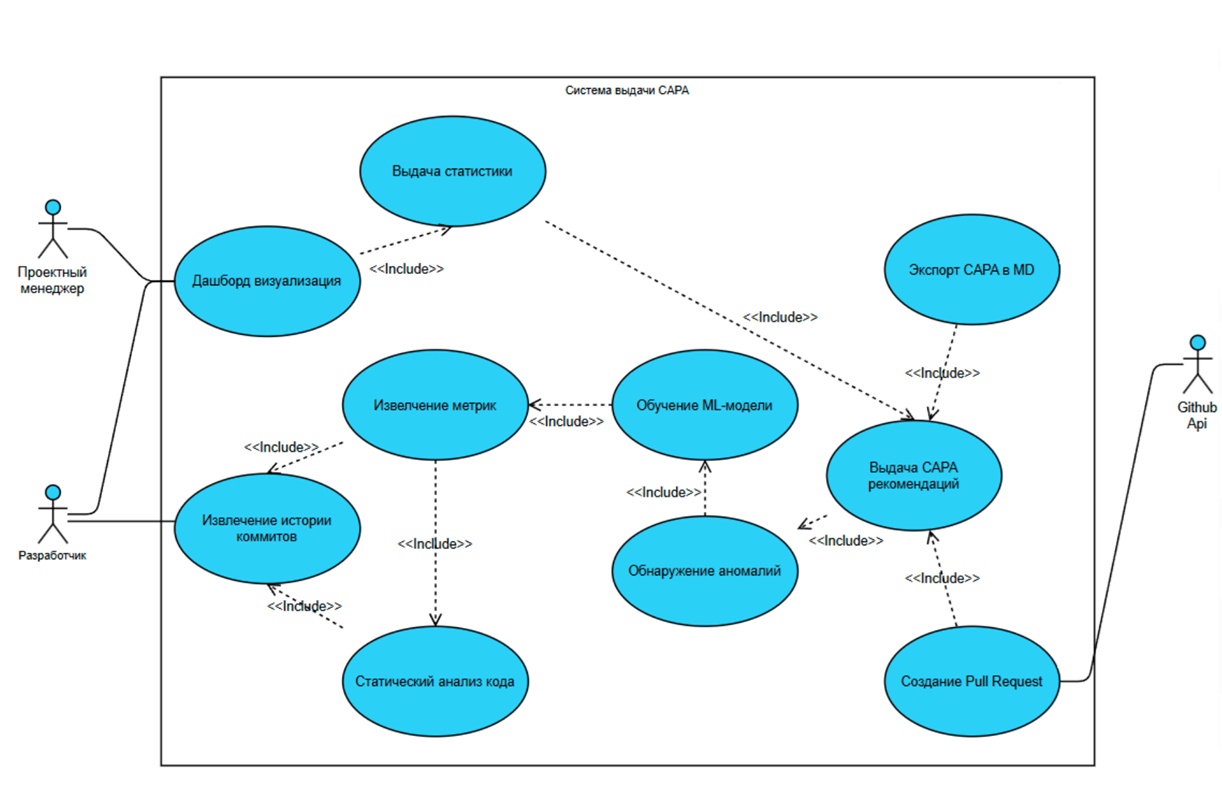
\includegraphics[width=0.9\textwidth]{my_folder/images/useCase (1).png}
	\caption{Use Case-диаграмма системы автоматического формирования CAPA}
	\label{fig:usecase}
\end{figure}


\section{Выводы} \label{ch1:conclusion}

Современные практики формирования CAPA на основе анализа репозиториев кода объединяют строгие процедуры управления качеством и динамическую ML-аналитику истории изменений. Классический цикл CAPA — сбор инцидентов, диагностика, планирование и проверка эффективности мер — дополняется JIT-предсказанием дефектов и классификацией коммитов на основе моделей машинного обучения, а также «бот-аналитикой» (TOM, GitHub Apps), когда система сама собирает метрики и создаёт pull-request’ы с рекомендациями. При выборе решения критичны автоматизируемость, интеграция в CI/CD, учёт истории коммитов и интерпретируемость результатов. Статические анализаторы (SonarQube) надёжно автоматизируются, но не отслеживают эволюцию проекта, а ML-модели улавливают сложные паттерны в истории, но требуют обучения и часто выступают «чёрным ящиком». Наименее работоспособным оказывается чистый QMS-софт без аналитики кода. Лучшие практики — это гибридный подход: статический анализ, ML-классификация и интеграция с баг-трекером для автосоздания задач CAPA.


